\section{Sleep inertia in high and low dream recallers}
\label{res:inertia:drf}

\bigskip

\textbf{{\large Brain functional connectivity upon awakening from sleep predicts between-subject differences in dream recall frequency}}

\hfill \emph{In preparation}

\bigskip

Raphael Vallat\textsuperscript{1} (PhD candidate), Alain Nicolas\textsuperscript{1,2} (M.D, PhD), Perrine Ruby\textsuperscript{1} (PhD)

\textsuperscript{1} Lyon Neuroscience Research Center, Brain Dynamics and Cognition team, INSERM UMRS 1028, CNRS UMR 5292, Université Claude Bernard Lyon 1, Université de Lyon, Lyon, France

\textsuperscript{2} Unité Michel Jouvet, Centre Hospitalier Le Vinatier, 95 boulevard Pinel, Lyon, France

\subsection*{Summary}
\label{res:inertia:drf:summary}

Dreaming is a fascinating and universal experience that remains still poorly understood. Perhaps one of its most intriguing aspect relates to why some people recall up to several dreams per day while some hardly ever recall one. Previous results suggest that memory performance during wake could not explain such inter-individual differences in dream recall but that the brain transitional state during sleep inertia immediately following awakening could . To test this hypothesis we designed a combined EEG-fMRI study. We aimed at investigating the brain functional connectivity of high dream recallers (HR, n=27) and low dream recallers (LR, n=27) in the minutes following awakening from a 45 min mid-afternoon nap. Resting-state scans were acquired before the nap, 5 min and 25 min after awakening and were each paired with a mental calculation task. Between-group contrasts of the functional connectivity at 5 min post-awakening revealed a pattern of enhanced connectivity in HR within the default mode network and regions involved in memory retrieval (i.e. medial prefrontal cortex, precuneus, left medial temporal lobe, left dorsolateral prefrontal cortex). These findings are discussed regarding the idea of a neurophysiological trait difference between HR and LR .


\paragraph{Keywords}
Dream recall, sleep inertia, awakening, EEG-fMRI, functional connectivity, default mode network

\subsection*{Introduction}
\label{res:inertia:drf:intro}

Dreaming is a universal and fascinating experience which happens most probably every night when we plunge into sleep. However, several aspects of dreaming are still poorly understood, among which is the large inter-individuals difference in dream recall frequency (DRF). Previous results demonstrated that intra-sleep wakefulness is one explaining factor of DRF variability \citep{eichenlaub_brain_2014, vallat_increased_2017}. However this factor does not explain everything since controlled awakenings in the lab still result in drastically more frequent dream recall in high dream recallers (HR) than in low dream recallers (LR) whatever the sleep stage \citep{goodenough_comparison_1959, eichenlaub_resting_2014, eichenlaub_brain_2014}.

Sleep inertia, the transient period following awakening and associated with impaired performances \citep{tassi_sleep_2000, trotti_waking_2016}, could be the missing link. Awakenings would enable the encoding of the dream into long term memory when the transition between sleep and wakefulness spare the short term memory of the dream \citep{koulack_dream_1976}. The hypothesis is thus that, compared to HR, LR would show more cognitive impairments and functional connectivity disturbances caused by sleep inertia in the first minutes following awakening from sleep. This hypothesis is supported by previous results which have shown functional brain differences between HR and LR using EEG \citep{eichenlaub_brain_2014} and PET \citep{eichenlaub_resting_2014}. As compared to LR, HR notably showed an increased regional cerebral blood flow (rCBF) in the medial prefrontal cortex (MPFC) and temporo-parietal junction (TPJ).

The proper functioning of these regions, known to be involved in dream production and/or recall (i.e. lesions of one or both of these regions induce a cessation of dream reports; \citealp{solms_neuropsychology_1997, solms_dreaming_2000}) could thus explain the successful retrieval of dream content upon awakening. Specifically, we postulate that the strength of the functional connectivity in the network comprising these two regions, namely the default mode network (DMN), is required to recall dreams at awakening. The DMN is a set of functionally coupled brain areas \citep{raichle_default_2001, legrand_what_2009, sestieri_episodic_2011} that are highly activated during mental imagery and episodic memory retrieval, and whose functional connectivity is diminished during sleep \citep{horovitz_decoupling_2009, larson-prior_modulation_2011, samann_development_2011}. Several authors have postulated that the DMN might be the brain network underlying the dreaming experience \citep{domhoff_neural_2011, christoff_mind-wandering_2016}.

The present study aims therefore at testing the hypothesis of a differential brain functioning of HR and LR specifically during the period following awakening from sleep. This hypothesis has surprisingly never been experimentally tested before, despite several studies mentioning the brain and cognitive functioning immediately upon awakening as a potential explaining factor of DRF variability \citep{schredl_factors_2003, conduit_poor_2004}. The period following awakening from sleep is a distinct and transient state that is measurably different from wakefulness since it is characterized by impaired performance, hypovigilance and sleepiness. We therefore hypothesized that sleep inertia and its cerebral correlates may account for the inter-individual differences in DRF. In other words we expected more impaired cognitive performances and functional connectivity at awakening in LR than in HR.

Several studies are consistent with this hypothesis. First, sleep inertia is higher following sleep deprivation or awakening from N3 sleep, which are both factors associated with a lower rate of dream recall \citep{nielsen_review_2000, de_gennaro_recovery_2010}. Second, \citet{conduit_poor_2004} found that memory abilities after awakening from N2 sleep were lower than after awakening from REM sleep, and that these impairments were significantly correlated with reported dream recall frequency (i.e. better memory performances and better dream recall after awakening from REM sleep).

To test our hypotheses, we designed a combined EEG-fMRI study. We aimed at investigating the brain functional connectivity in the minutes following awakening from a 45 minutes mid-afternoon nap in HR vs LR. Resting-state scans were acquired before the nap, 5 min and 25 min after awakening to investigate the dynamics of brain functional reorganization during the first half hour following awakening, and each scan was associated with a mental calculation task to measure the cognitive impairments of sleep inertia. We predicted that HR would show (1) more dream recall following awakening from sleep (2) a higher functional connectivity within the DMN and between regions involved in memory retrieval (3) less cognitive performance impairments, suggesting a faster recovery of normal cognitive functioning upon awakening.

\subsection*{Methods}
\label{res:inertia:drf:methods}

\subsubsection*{Participants}
Behavioral and neurophysiological data were acquired from 55 healthy subjects (28 males, mean age = 22.55, standard deviation = 2.41, range = 19–29). The subjects were informed of the study through an announcement sent to the mailing list of Lyon University, which briefly described the study and included a link to a questionnaire concerning sleep and dream habits. Subjects were selected if they reported and subsequently confirmed during a phone interview: (1) having a high or low DRF (DRF superior to 5 dream recalls per week and inferior to 2 dream recalls per month respectively) (2) having a regular sleep-wake schedule, no difficulty to fall asleep, being occasional or frequent nappers and having preferentially already done an MRI brain scan in the past few years. Importantly, the subjects were unaware that DRF was the main criterion for inclusion in the study. Among the 55 participants, 28 of them were high dream recallers (HR; mean DRF = 6.6 ± 0.7 dream reports per week) and 27 were low dream recallers (LR; mean DRF = 0.2 ± 0.1 dream report per week). Apart from the DRF (p < .001), the two groups did not differ in age, habitual sleep duration or education level (see Table 1 of section \ref{res:dmn-crea:results}). They had no history of neurological and psychiatric disorders, and had no sleep disturbances. They provided written informed consent according to the Declaration of Helsinki and received monetary compensation for their participation. The study was approved by the local ethics committee (CCPPRB, Centre Leon Berard, Lyon, France).

\subsubsection*{Behavioral tests}
The night before the experiment, the subjects underwent a partial sleep deprivation (they were allowed to sleep between 5 am and 8 am; see Procedure). Between 9 pm and 11 pm, the subjects were presented with various tests to assess the potential between group differences at the cognitive and personality levels, the results of which will be detailed elsewhere.

In addition, participants trained on the descending subtraction task (DST), which was used to evaluate cognitive performances during the MRI session on the following day, in order to avoid a practice effect over the first trials \citep{dinges_assessing_1985}. The DST has been previously used to evidence performances decrement and normalization in the first 30 min post awakening \citep{evans_recovery_1975, dinges_assessing_1985, stampi_ultrashort_1990}. Subjects were presented with a three-digit number. They were instructed to subtract 9, saying the operation and the result aloud, and then continue by subtracting 8 from the remainder, then 7, and so on until they had to subtract 1. At this point they were to start the cycle of descending subtractions again. They had to do the task for two minutes and were instructed to be as fast and accurate as possible.

\subsubsection*{Procedure}
\emph{Evening and night}. To facilitate sleep in the MRI environment, participants underwent a 3 h partial sleep deprivation on the night before the experiment. Specifically, they arrived in the sleep unit of the hospital Le Vinatier (Lyon, France) at 8 pm. During two hours they performed the previously described personality and cognitive tests, administered by R.V. They were then instructed to stay awake until 5 am (the possible activities were reading, making puzzles and watching movies), at which point they were allowed to sleep for 3 hours until 8 am in a bed in the sleep unit. Energy drinks or physical activity were prohibited during the partial sleep deprivation, and nurses regularly checked that the subject did not fall asleep. The monitoring of body movements through wrist actigraphy (Actigraph, Pensacola, USA) during the whole night made it possible to check a posteriori that the subject did not fall asleep before 5 am. In the morning, participants were offered breakfast and a shower and then occupied themselves (reading or internet) under the experimenters’ supervision until the MRI session.

\emph{Day}. The MRI procedure is shown in Fig \ref{fig:intro:problematics-fmri-paradigm}. After lunch at 11.30 am, participants were conducted to the neuroimaging center (CERMEP). During the first half hour, experimenters installed on the participant’s head a MRI compatible EEG cap (EASYCAP®). Participants were then installed in the MRI scanner at about 1.20 pm (1.17 pm ± 13 min). They read a 5 min cartoon during the calibration of the eye-tracking camera, and then performed the descending subtraction task (DST) for 2 minutes. The first resting-state scan was then acquired, with the instructions to remain awake and look at a central fixation cross on the screen. At the end of the scan, participants were informed that they could sleep (at 1.39 pm ± 14 min in average) during the next 45 min. At the end of the nap slot, participants were awakened, if they were sleeping, by calling their first name and the 2nd resting state scan was acquired. At the end of the scan, the 2nd DST was performed. During the following 10 minutes, subjects were asked about their dream(s) and sleep in the scanner and about the cartoon. Then the 3rd resting state scan and DST were performed (about 25 min after awakening). Finally, an 8-min T1 anatomical scan was acquired.

\subsubsection*{Data collection}
\paragraph{EEG and eye movement recordings}
Polysomnography data was recorded using a 15 channels MR-compatible cap designed for sleep studies i.e. with a layout designed according to American Academy of Sleep Medicine Guidelines 2007 (EasyCap, Brain Products GmbH, Gilching, Germany). It comprised 9 EEG electrodes placed according to the international standard 10/20 system (O1, O2, C3, C4, F3, F4, M1, M2, Cz, FCz was used as reference and AFz as ground), 2 EOG electrodes, 3 EMG electrodes, and an electrocardiogram electrode placed on the back of the participant. The sampling rate was 5000 Hz and an analog band-pass filter was set to 0.01 – 250 Hz.  To score sleep online during the fMRI session, a real-time pulse-artefact correction was performed using the BrainVision Recorder (Version 1.2) and BrainVision RecView (Version 1.4) softwares (Brain Products).

To ensure that participants were not closing their eyes during the resting state scans, eye movements were monitored during the experiment using an EyeLink 1000 fMRI eye tracking system (SR Research Ontario, Canada). Eye position was calibrated at the beginning of the experiment and monitored throughout.

\paragraph{MRI acquisition}
MRI scans were obtained from a MAGNETOM Prisma 3.0 T scanner (Siemens Healthcare, Erlangen, Germany) at the Primage neuroimaging platform (CERMEP). Structural MRI were acquired with a T1-weighted (0.9-mm isotropic resolution) MPRAGE sequence and functional MRI data with a T2*-weighted 2D gradient echo planar imaging sequence (EPI) with 180 volumes (TR/TE: 2000/ 25 ms; flip angle: 80°; voxel size: 2.68 × 2.68 × 3 mm; slices: 40, duration: 6 minutes). Functional and anatomical scans were performed using a 20-channel head coil. The coil was foam-padded to improve subject comfort and restrict head motion.

\subsubsection*{Data analysis}
\paragraph{EEG}
Artifacts related to gradient switching and cardiac pulse (cardio-ballistic artifact) were removed using standard routines available in BrainVision Analyzer version 2.0 software (Brain Products). Polysomnographic data were downsampled to 1000 Hz and band-pass filtered between 0.5 and 25 Hz. Offline sleep stage scoring was performed using EEG epochs of 30 seconds following standard AASM rules \citep{iber_aasm_2007} visualized using SLEEP software \citep{combrisson_sleep:_2017}.

\paragraph{fMRI}
Preprocessing and quality check were performed using standard routine in SPM12 software (Wellcome Department of Imaging Neuroscience). Preprocessing included functional realignment, slice-time correction, coregistration to structural scan, spatial normalization and spatial smoothing using a 6 mm full-width at half-maximum isotropic Gaussian kernel filter. Individual T1 images were segmented into gray matter, white matter and cerebrospinal fluid tissue maps. Functional and structural images were then normalized to MNI152 space (Montreal Neurological Institute). Functional images underwent artifact and motion regression in the ART toolbox using the following criteria to define outliers: global signal intensity changes greater than 9 standard deviations and movement exceeding 2 mm. SPM motions parameters and outliers were subsequently included as covariates in connectivity analyses.

Connectivity analysis were performed using the CONN toolbox version 17f. First, we performed a denoising step including a regression of the 6 motion correction parameters and their corresponding first-order temporal derivatives, as well as a component-based strategy (aCompCor, \citealp{behzadi_component_2007}) to identify and remove physiological confounds that are unlikely to be related to neural activity. The resulting BOLD time series were band-pass filtered (0.008 – 0.09 Hz) to further reduce noise and increase sensitivity \citep{weissenbacher_correlations_2009}. We then performed seed-to-voxel analysis using a seed in the medial prefrontal cortex (MPFC; center of mass in MNI coordinates: 1, 55, -3), one core region of the DMN which is critically involved in dream recall \citep{solms_neuropsychology_1997, eichenlaub_brain_2014}.

\paragraph{Statistics}
For the DST, between-group comparisons were achieved using a mixed two-way repeated measures ANOVA with a group factor (two levels: HR and LR) and a time factor (within subject factor with three levels: Pre-sleep, 5 min p-a, 25 min p-a). Post hoc analyses (t-tests) were used in case of significance. Seed-based connectivity analysis were performed using a cluster-defining voxel-wise height threshold of p<.01 (uncorrected, two-sided) and a whole-brain family-wise error (FWE) corrected extent threshold of p<.05.

\subsection*{Results}
\label{res:inertia:drf:results}

\subsubsection*{Sleep parameters}
As expected and due to the inherent discomfort of the MRI environment, 11 out of 55 participants were not able to reach N2 sleep during the 45 min nap slot. One subject out of the 44 remaining was discarded because of a technical failure during data acquisition, leading thus to a total of 43 participants included in the final analysis (21 HR, 22 LR). Means of the main sleep parameters in the two groups are presented in Table 1. Importantly, there was no significant group difference for any of the sleep parameters considered or in the latency between the awakening and the two post-awakening resting-state scans.

\begin{table}[!htbp]
    \caption*{\textbf{Table 1. Mean sleep parameters of the HR (n=21) and LR (n=22) groups.} TST = Total Sleep Time, SE = Sleep Efficiency, Wake (W), N1, N2 and N3 = Total duration of each sleep stage in minutes. LAS1 = latency (min) between the awakening and the start of the first post-awakening resting-state scan. LAS2 = latency (min) between the awakening and the start of the second post-awakening resting-state scan. N.S = not significant.}
    \begin{tabularx}{\textwidth}{lXXXXXXXX}
    \toprule
    Group  & TST          & SE (\%)      & W            & N1           & N2           & N3           & LAS1         & LAS2         \\ \midrule
    HR     & 35.6         & 85.7         & 9.3          & 12.9         & 16.8         & 6.3          & 3.4          & 24.3         \\
    SD     & 8.4          & 11.9         & 5.0          & 7.9          & 5.6          & 6.4          & 1.0          & 4.2          \\
    LR     & 36.3         & 83.6         & 11.2         & 11.5         & 18.7         & 6.4          & 4.8          & 23.5         \\
    SD     & 6.3          & 11.7         & 5.2          & 6.9          & 7.3          & 6.0          & 4.0          & 3.6          \\
    T-test & \textit{N.S} & \textit{N.S} & \textit{N.S} & \textit{N.S} & \textit{N.S} & \textit{N.S} & \textit{N.S} & \textit{N.S} \\ \bottomrule
    \end{tabularx}%
\end{table}

\subsubsection*{Behavioral results}
\paragraph{DST}
DST performances are reported in S2 Fig. A two-way ANOVA revealed a significant effect of time in the number of responses (F(2, 41) = 7.44, p = .001) and percentage of correct responses (F(2, 41) = 5.03, p = .009) compared to pre-nap performances.  Specifically, the total number of responses was reduced at 5 min p-a compared to pre-nap and 25 min p-a (p = .003 and p < .001, respectively). There was no main effect of time in the percentage of mistakes, a finding in line with the generally held view that speed is more impaired than accuracy during sleep inertia \citep{trotti_waking_2016}. Most importantly, there was no main effect of group or interaction between group and time for any of the three outcome measures considered. Sleep inertia, as measured by the DST, did not differ between the two groups.

\paragraph{Dream recall}
After awakening from the partial sleep deprivation in the sleep unit, more HR reported dreams than did LR (64\% of HR and 19\% of LR reported a full or a white dream). This was also the case after awakening from the 45 min nap inside the MRI (76\% of HR versus 36\% of LR).

\subsubsection*{Functional connectivity}
The results of functional connectivity contrasts between HR and LR in the three resting-state scans are presented in Fig 1 and Table 2. First, and perhaps most importantly, we found that during the resting-state scan conducted 5 min after awakening from NREM sleep, HR demonstrated an increased functional connectivity between the MPFC and other core regions of the DMN, including the precuneus and temporal fusiform cortex, and between the MPFC and dorsolateral prefrontal cortex (DLPFC). Second, at 25 min post-awakening, seed-based analysis revealed an increased functional connectivity in HR between the MPFC and caudate nucleus. No between-group differences were found during the pre-sleep resting-state scan.

\begin{figure}[!htbp]
	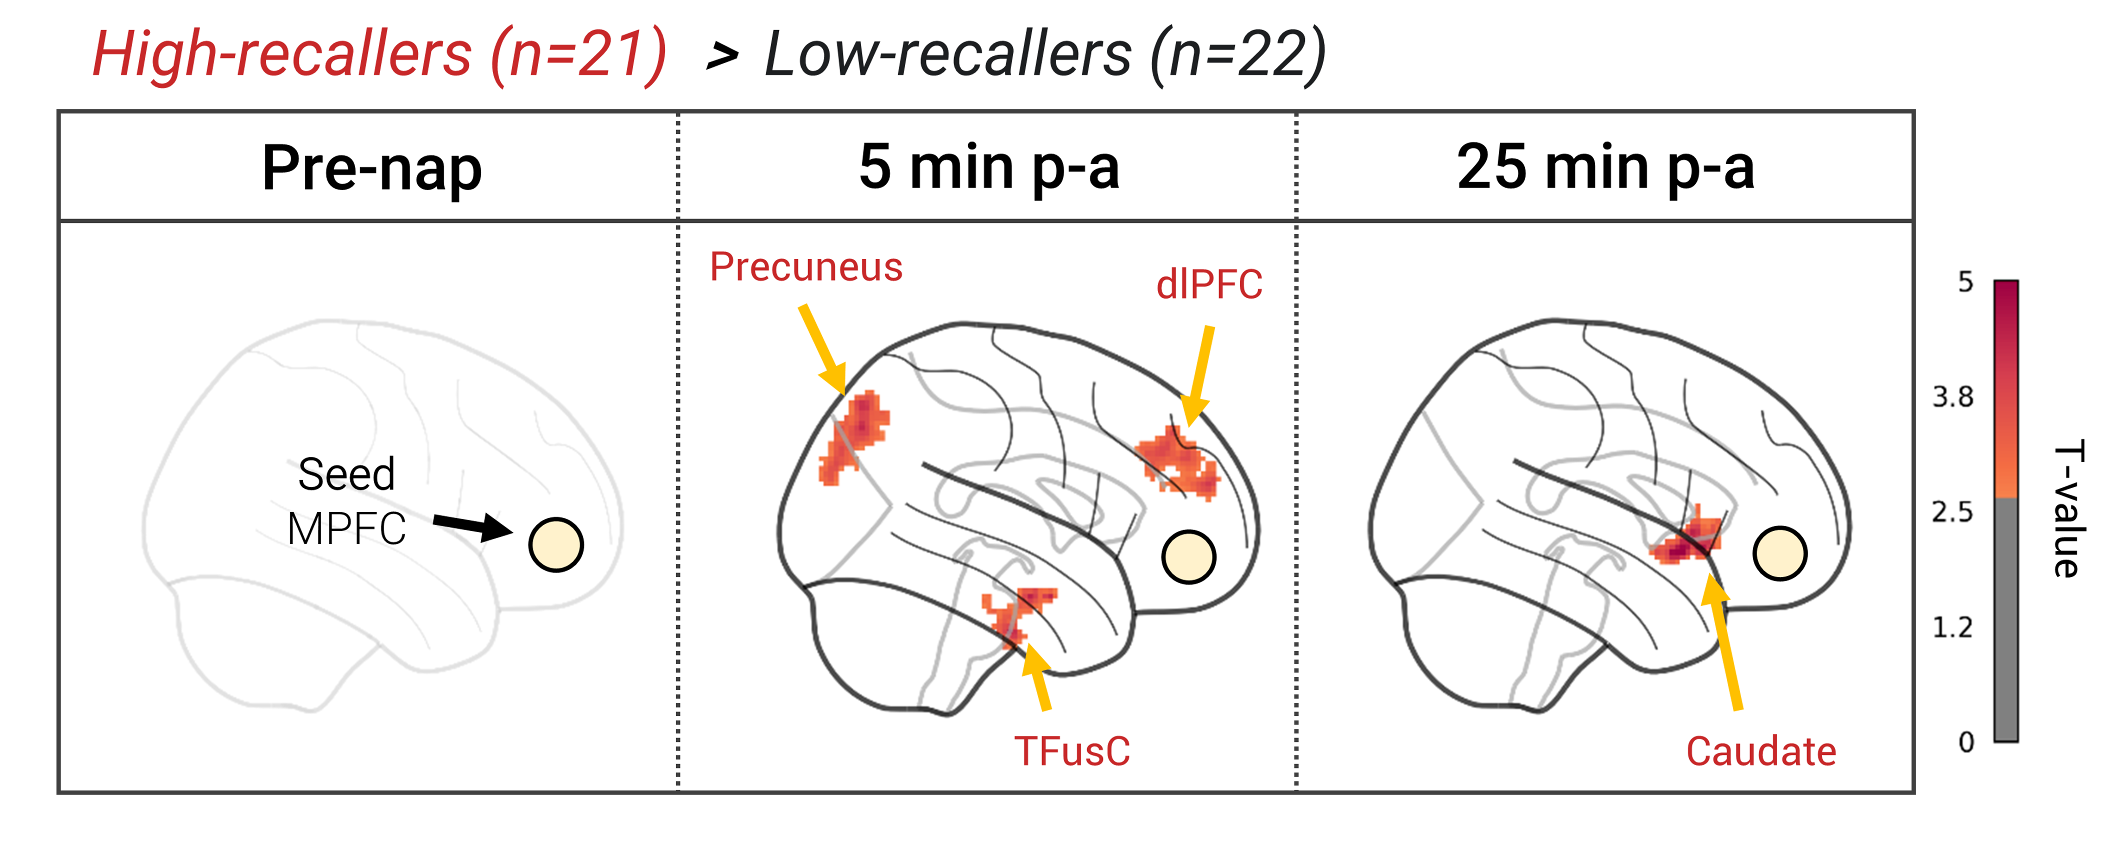
\includegraphics[width=\textwidth]{Fig/Results/Inertia/DRF/Fig1.png}
	\caption*{\textbf{Fig 1. Functional connectivity differences between High-recallers (HR) and Low-recallers (LR) during pre-sleep scan, 5 min post-awakening scan and 25 min post-awakening scan.} Seed-based connectivity results showing foci with higher activation in HR than in LR. Seed region (yellow circle) is the medial prefrontal cortex (MPFC, center of mass in MNI coordinates: 1, 55, -3), a region critically involved in dream recall. Statistical parametric maps are superimposed on a glass brain using an uncorrected two-sided cluster-defining voxel-wise height threshold of p<.01 and a whole-brain FWE-corrected extent threshold of p<.05. MPFC = medial prefrontal cortex, dlPFC = dorsolateral prefrontal cortex, TFusC = temporal fusiform cortex. Faded brain denotes an absence of significant differences between the two groups.}
\end{figure}

\begin{table}[!htbp]
    \caption*{\textbf{Table 2. Seed-based functional connectivity results for the group comparison (HR (n=21) minus LR (n=22))}. Seed region (black circle) is the medial prefrontal cortex (MPFC, center of mass in MNI coordinates = 1, 55, -3). Statistical analyses were performed using a cluster-defining voxel-wise height threshold of p<.01 (uncorrected, two-sided) and a whole-brain family-wise error (FWE) corrected extent threshold of p<.05.}
    \begin{tabularx}{\textwidth}{lXlllXX}
    \toprule
                &              & \multicolumn{3}{l}{MNI coordinates} &              &              \\
    Scan        & Brain region & X          & Y          & Z         & T value      & Cluster size \\ \midrule
    Pre-sleep   & \textit{N.S} & -          & -          & -         & -            & -            \\
    5 min p-a   & Precuneous L & -6         & -76        & 42        & 4.97         & 512          \\
                & DLPFC L      & -34        & 60         & 20        & 4.86         & 356          \\
                & TFC L        & -40        & -18        & -38       & 5.49         & 251          \\
    25 min p-a  & Caudate R    & 14         & 12         & -8        & 6.01         & 277          \\ \bottomrule
    \end{tabularx}
\end{table}

\subsection*{Discussion}
\label{res:inertia:drf:discussion}

This study is the first to compare the brain functional connectivity and cognitive performances of high and low dream recallers in the minutes following awakening from sleep, in an effort to understand the basis for these individual differences in dream recall. The main findings are the followings. First, as expected significantly more HR reported a dream upon awakening than LR. Second, compared to LR, the brain functional connectivity of HR at 5 min post-awakening was significantly increased in several regions that all have in common to be involved in memory processes. Third, the arithmetic performances of both HR and LR were significantly impaired at 5 min post-awakening compared to pre-nap and 25 min post awakening, but no between group differences was observed. The significance of these findings is discussed below.

Between-group contrasts of the functional connectivity at 5 min post-awakening revealed a pattern of enhanced connectivity in HR within the DMN (namely the precuneus, medial prefrontal cortex and left medial temporal lobe) and between the DMN and the left DLPFC. Remarkably, all these regions have been associated with memory processes. In a meta-analysis of the brain areas associated with episodic encoding and retrieval, \citet{spaniol_event-related_2009} reported that the largest clusters associated with retrieval success were located in the precuneus, the anterior prefrontal cortex, the left DLPFC and, to a lesser extent, the middle temporal gyrus. These are almost exactly the same regions found to be more functionally connected in HR than LR during the first minutes following awakening.

Based on these findings, one may conclude that HR were deliberately involved in memory retrieval during the resting-state scans, hence an increase functional connectivity in these specific regions. This hypothesis is however unlikely given that subjects were asked to remember the content of their dreams only during the interval between the 5 min and 25 min post-awakening scans. Moreover, only 5 subjects (4 HR) reported that they were actively trying to recall the content of their dreams during the 5 min post-awakening scan.  Another possible interpretation is that these results reflect neurophysiological trait differences rather than strategy/task differences between HR and LR. This interpretation is supported by previous results showing, in HR, increased brain responses to auditory stimuli during wakefulness and sleep \citep{eichenlaub_brain_2014}, and increased regional cerebral blood flow in the MPFC and TPJ, also during sleep and wakefulness \citep{eichenlaub_resting_2014}. Since it is generally admitted that sleep inertia interferes with memory retrieval on awakening rather than memory consolidation \citep{bonnet_memory_1983, dinges_are_1990, tassi_sleep_2000, conduit_poor_2004}, the findings of the present study support the hypothesis of a differential brain functional organization upon awakening between HR and LR.  Specifically, increased functional connectivity between regions involved in memory retrieval would facilitate dream recall in HR, while decreased connectivity in those same regions would prevent successful dream recall in LR. These results suggest that the difference in DRF between HR and LR is not the result of a differential production of dreams, but rather of a differential recall of dreams upon awakening .

\subsubsection{Limitations}
First, the present study reported the brain functional connectivity of HR and LR following awakening from sleep stages, namely N2 and N3 sleep. It would be interesting to extend these data to N1 sleep and REM sleep. This latter, which has traditionally been viewed as the neural substrate of dreaming, is however very difficult to observe in an fMRI setting, unless applying a severe and specific REM sleep deprivation in the night(s) before \citep{duyn_eeg-fmri_2012}, which is of course not ideal to study functional connectivity given the huge impact of severe sleep deprivation on the brain functional connectome \citep{de_havas_sleep_2012, yeo_functional_2015, krause_sleep-deprived_2017}. Given the higher rate of dream recall following REM sleep than any other sleep stages \citep{nielsen_review_2000, ruby_experimental_2011}, one would expect that the functional connectivity between regions involved in memory retrieval would be higher following awakening from REM sleep than NREM sleep. This would in turn explain the better cognitive and memory performances (i.e. lesser sleep inertia) following REM sleep than NREM sleep \citep{bonnet_memory_1983, koukkou_dreaming:_1983, conduit_poor_2004}.

On another note, we were not able to evidence between-group differences in cognitive performances, measured by the DST, at 5 min post-awakening. There are two possible reasons for this. First, the DST was not performed immediately after awakening but after the 6 min resting-state scans, because we choose to favor the estimation of functional connectivity rather than cognitive performances directly upon awakening. \citet{bonnet_memory_1983} reported that the impairment of cognitive and memory performance upon awakening decreases as a function of time awake. Therefore the delay between awakening and the DST could account for a relatively small decrease in performance compared to pre-nap performances and the absence of group main effect. Second, while the DST has been previously reported to be affected by sleep inertia \citep{dinges_assessing_1985}, it is possible that this arithmetic task do not capture well the brain functioning and dream recall differences between HR and LR, as would have for instance a task more-specifically designed to assess memory retrieval.

\subsubsection{Conclusion}
The present study showed that inter-individual differences in dream recall frequency are associated with a differential brain functional connectivity in the minutes following awakening. Specifically, a higher functional connectivity between regions involved in memory retrieval just after awakening could facilitate in HR the retrieval of pre-awakening experiences and thus promote dream recall. More broadly, these results contribute to the growing body of evidence that trait differences in dream recall are supported by trait neurophysiological correlates. Further work is needed to better delineate the interactions between neurophysiological factors, psychological factors and inter-individual differences in dream recall.

% \paragraph{Acknowledgments}
% The authors would like to thank Basak Turker, Morgane Hamon, Franck Lamberton and Danielle Ibarrola for substantial help in data collection and analysis, as well as Jamila Lagha for her help in administrative work.
%
% \paragraph{Author contribution}
% R.V and P.R designed the study, acquired the data and wrote the paper. A.N participated to the design and provided access to his sleep unit to conduct the sleep deprivation.

\FloatBarrier

\subsection*{Supplementary materials}

S1 Fig is a duplicate of Fig \ref{fig:intro:problematics-fmri-paradigm} of the present thesis.

S1 table is a duplicate of Table 1 Study 3 (section \ref{res:dmn-crea:results}).

\vspace*{1cm}

\begin{figure}[!htbp]
	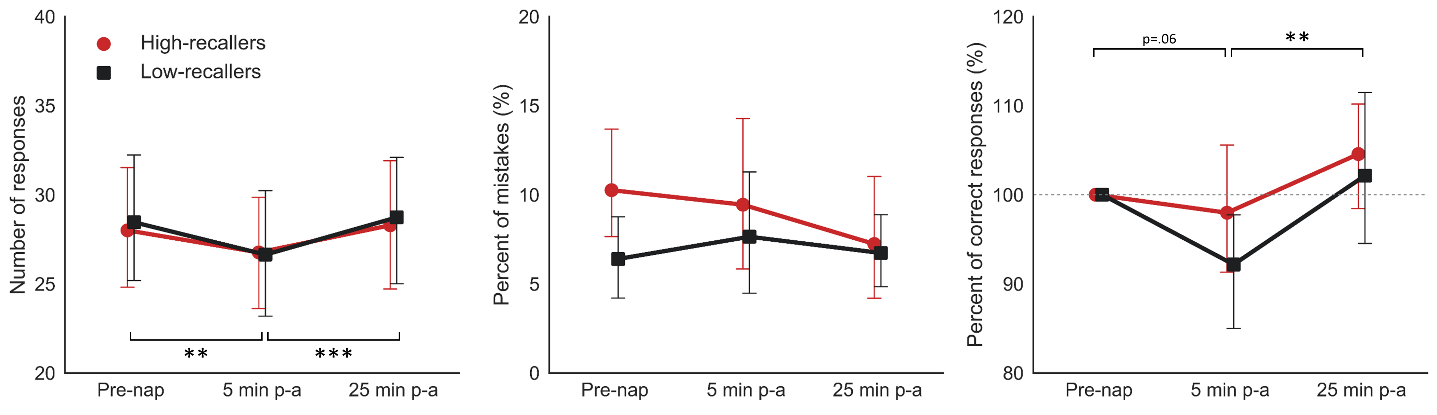
\includegraphics[width=\textwidth]{Fig/Results/Inertia/DRF/S2_Fig.png}
	\caption*{\textbf{S2 Fig. Performances of the Descending Subtraction Task.} Red lines, High-recallers (n=21), black lines, Low-recallers (n=22). (A) Total number of responses (index of speed). (B) Percentage of mistakes (marker of accuracy). (C) Percentage of correct responses relative to pre-nap performances (marker of both speed and accuracy). Error bars represent 95\% confidence intervals. * p<.05, *** p<.001}
\end{figure}
